%%%%%%%%%%%%%%%%%%%%%%%%%%%%%%%%%%%%%%%%%%%%%%%%%%%%%%%%%%%%%%%%%%%%%%%%%%%%%%%%%%%%%%%%%%%%%%%%%%%%%
%Include files, leave this alone
\title{CS18 HW6.4 analysis}

\documentclass[12pt,letterpaper]{article}
\usepackage{amsmath}
\usepackage{algpseudocode}
\usepackage{tikz}
\usepackage{cancel}
\usetikzlibrary{arrows}
\usepackage{fullpage}
\usepackage{enumerate}
\usepackage{fancyhdr}
\setlength{\parindent}{0.0in}
\setlength{\parskip}{0.1in}
\newcommand{\tab}{\hspace{3em}}
%%%%%%%%%%%%%%%%%%%%%%%%%%%%%%%%%%%%%%%%%%%%%%%%%%%%%%%%%%%%%%%%%%%%%%%%%%%%%%%%%%%%%%%%%%%%%%%%%%%%%


% Edit these as appropriate
\newcommand\course{CS 18}
\newcommand\semester{Spring 2014}       % <-- current semester
\newcommand\hwnum{8}                  % <-- homework number

%%%%%%%%%%%%%%%%%%%%%%%%%%%%%%%%%%%%%%%%%%%%%%%%%%%%%%%%%%%%%%%%%%%%%%%%%%%%%%%%%%%%%%%%%%%%%%%%%%%%%
%This section setups the header for the document, leave this alone
\pagestyle{fancy}
\headheight 28pt
\fancyhead[R]{\course, \semester\\ Homework \hwnum, \today}
%%%%%%%%%%%%%%%%%%%%%%%%%%%%%%%%%%%%%%%%%%%%%%%%%%%%%%%%%%%%%%%%%%%%%%%%%%%%%%%%%%%%%%%%%%%%%%%%%%%%%

\newenvironment{answer}[1]{
  \section*{Problem \hwnum.#1}
}{\newpage}

%%%%%%%%%%%%%%%%%%%%%%%%%%%%%%%%%%%%%%%%%%%%%%%%%%%%%%%%%%%%%%%%%%%%%%%%%%%%%%%%%%%%%%%%%%%%%%%%%%%%%
%The document begins here!
\begin{document}

\newcommand{\tabb}[1]{\hspace{.2\textwidth}\rlap{#1}}

\begin{answer}{4}

\textbf{Longest Path} \\

\begin{algorithmic}
\tt{

	\Require a DAG $(V, E)$ and a source node $s$
	\Ensure a $distance$ array, stores the longest distance to each vertex $v$ from $s$
    \Function{SSLP}{$V, E, s$}
	\For{$v \in V$}
    	\State $distance[v] \leftarrow -\infty$
    \EndFor
    \State $distance[s] \leftarrow 0$
    \State $V^* = V$, sorted in topological order
	\For {$v \in V^*$}
    	\For{$u|(u,v) \in E$}
        \State $distance[v] \leftarrow max\{distance[v], distance[u] + w(u,v)\}$
        \EndFor
    \EndFor
\EndFunction
}
\end{algorithmic}

\begin{verbatim}






















\end{verbatim}

\textbf{Longest Path Dijkstra's} \\

\begin{algorithmic}
\tt{

	\Require a graph $(V, E)$ and a source node $s$
	\Ensure a $distance$ array, stores the longest distance to each vertex $v$ from $s$
    \Function{SSLP}{$V, E, s$}
    \State $PQ$ = max-heap priority queue
	\For{$v \in V \backslash \{s\}$}
    	\State $distance[v] \leftarrow -\infty$
        \State $PQ$.\Call {insert}{$v, distance[v]$}
    \EndFor
    \State $distance[s] \leftarrow 0$
    \State $PQ$.\Call {insert}{$s, distance[s]$}
	\While {$\neg PQ.$\Call{isEmpty}{}()}
    	\State $u \leftarrow PQ.$\Call{deleteMax}{}()
    	\For{$u|(u,v) \in E$}
        \If{$distance[v] < distance[u] + w(u, v)$}
        	\State $distance[v] \leftarrow distance[u] + w(u, v)$
            \State $parent[v] \leftarrow u$
            \State $PQ.$\Call{increaseKey}{$v, distance[v]$}
        \EndIf
        \EndFor
    \EndWhile
\EndFunction
}
\end{algorithmic}

The above algorithm does not give the longest paths in a cyclic graph. Consider the graph in fig. 1.

fig 1.
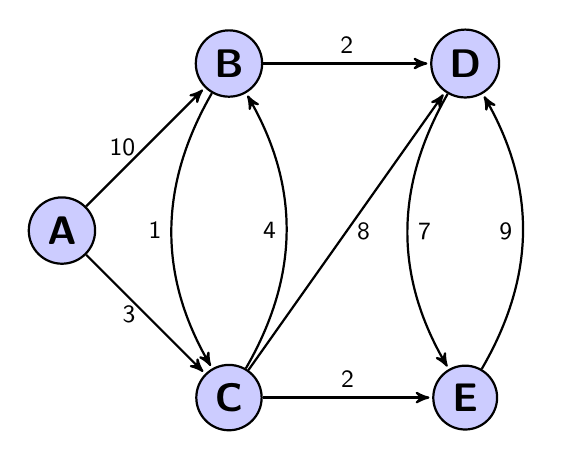
\begin{tikzpicture}[->,>=stealth',shorten >=1pt,auto,node distance=3cm,
  thick,main node/.style={circle,fill=blue!20,draw,font=\sffamily\Large\bfseries}]

  \node[main node] (A) {A};
  \node[main node] (B) [above right of=A] {B};
  \node[main node] (C) [below right of=A] {C};
  \node[main node] (D) [right of=B] {D};
  \node[main node] (E) [right of=C] {E};

  \path[every node/.style={font=\sffamily\small}]
    (A) edge node [left] {10} (B)
        edge [right] node[left] {3} (C)
    (B) edge [bend right] node[left] {1} (C)
        edge [right] node[above] {2} (D)
    (C) edge [bend right] node[left] {4} (B)
        edge [right] node[right] {8} (D)
        edge [right] node[above] {2} (E)
    (D) edge [bend right] node [right]{7} (E)
    (E) edge [bend right] node [left] {9} (D);
\end{tikzpicture}

Following this algorithm would result in the following steps:\\\\\\\\\\

\begin{tabular}{c|c|c|c|c||c}
A & B & C & D & E & PQ \\ \hline
0 & $- \infty$ & $- \infty$ &$- \infty$ &$- \infty$ & $A_0 B_{- \infty} C_{- \infty} D_{- \infty} E_{- \infty}$ \\

0 & 10 & 3 &$- \infty$ &$- \infty$ & $\cancel{A_0} B_{- \infty} C_{- \infty} D_{- \infty} E_{- \infty}$ \\

0 & 10 & 11 & 12 &$- \infty$ & $\cancel{B_{10}} C_{3} D_{- \infty} E_{- \infty}$ \\

0 & 10 & 11 & 12 & 19 & $\cancel{D_{12}} C_{11} E_{- \infty}$ \\

0 & 10 & 11 & 21 & 19 & $\cancel{E_{19}} C_{11}$ \\

0 & 10 & 11 & 21 & 19 & $\cancel{C_{11}}$ \\

\end{tabular}




The values in the distance array in the bottom row when the algorithm terminates are not the longest paths. For instance, the longest distance to D is 22, along the path A-B-C-E-D. The other problem is that the algorithm does not find a simple path. The distance found in the array for D, 21, is  from the path A-B-D-E-D, which passes through D twice.























\end{answer}

\end{document}